\documentclass[12pt]{report}

\usepackage[utf8]{inputenc}
%\usepackage[T1]{fontenc}
%\usepackage[français]{babel}
\usepackage{color}
\usepackage[OT1]{fontenc}
%\usepackage{lipsum}
\usepackage{graphicx}
\usepackage{geometry}
\usepackage[colorlinks=true,breaklinks=true,linkcolor=blue]{hyperref} 
%--------------------------------------------------------------
%--------------------------------------------------------------
\usepackage{listings}
%\definecolor{darkWhite}{rgb}{0.94,0.94,0.94}
%\definecolor{darkWhite}{rgb}{0.94,0.94,0.94}
\lstset{
	aboveskip=3mm,
	belowskip=-2mm,
	backgroundcolor=\color{white},
	basicstyle=\footnotesize,
	breakatwhitespace=false,
	breaklines=true,
	captionpos=b,
	commentstyle=\color{red},
	deletekeywords={...},
	escapeinside={\%*}{*)},
	extendedchars=true,
	framexleftmargin=16pt,
	framextopmargin=3pt,
	framexbottommargin=6pt,
	frame=tb,
	keepspaces=true,
	keywordstyle=\color{blue},
	language=C,
	literate=
	{²}{{\textsuperscript{2}}}1
	{⁴}{{\textsuperscript{4}}}1
	{⁶}{{\textsuperscript{6}}}1
	{⁸}{{\textsuperscript{8}}}1
	{€}{{\euro{}}}1
	{é}{{\'e}}1
	{è}{{\`{e}}}1
	{ê}{{\^{e}}}1
	{ë}{{\¨{e}}}1
	{É}{{\'{E}}}1
	{Ê}{{\^{E}}}1
	{û}{{\^{u}}}1
	{ù}{{\`{u}}}1
	{â}{{\^{a}}}1
	{à}{{\`{a}}}1
	{á}{{\'{a}}}1
	{ã}{{\~{a}}}1
	{Á}{{\'{A}}}1
	{Â}{{\^{A}}}1
	{Ã}{{\~{A}}}1
	{ç}{{\c{c}}}1
	{Ç}{{\c{C}}}1
	{õ}{{\~{o}}}1
	{ó}{{\'{o}}}1
	{ô}{{\^{o}}}1
	{Õ}{{\~{O}}}1
	{Ó}{{\'{O}}}1
	{Ô}{{\^{O}}}1
	{î}{{\^{i}}}1
	{Î}{{\^{I}}}1
	{í}{{\'{i}}}1
	{Í}{{\~{Í}}}1,
	morekeywords={*,...},
	numbers=left,
	numbersep=10pt,
	numberstyle=\tiny\color{black},
	rulecolor=\color{black},
	showspaces=false,
	showstringspaces=false,
	showtabs=false,
	stepnumber=1,
	stringstyle=\color{cyan},
	tabsize=4,
	title=\lstname,
	basicstyle=\tiny,
}

%------------------------------------------------------------------------------
%------------------------------------------------------------------------------

\geometry{verbose, letterpaper, tmargin=20mm, bmargin=20mm, lmargin=20mm, rmargin=20mm}
%\renewcommand\thechapter{\Roman{chapter}}
\renewcommand\thesection{\Roman{section}}
%\renewcommand\thesubsection{\roman{section}}
\renewcommand\contentsname{\bf \Large \sc Table des Matières}

% \texttt commande comme les 

\begin{document}
	\thispagestyle{empty}
%	\contentsname{KKKK}
	\begin{center}
		\textsc{\large Université d'Abomey-Calavi}             							  		\\ \vspace{3em}  %vfill
		\textsc{\Large Institut de Mathématiques et de Sciences Physiques}                   	\\ \vspace{2em}
		
		
		\rule{0.90\textwidth}{1.67pt}																\\ \vspace{1.2em}

		\textsc{\large Travaux Pratiques Big Data} 	
		
							  		
%		\rule{0.90 \textwidth}{2pt}					
		\vspace{3em}			
		\textsc{\Large Développement d'une Plateforme de Troc d'Objets} 	\\ 
		
		\vspace{2em}
	
		\textsc{Master I - Informatique}
		
			\begin{center}
				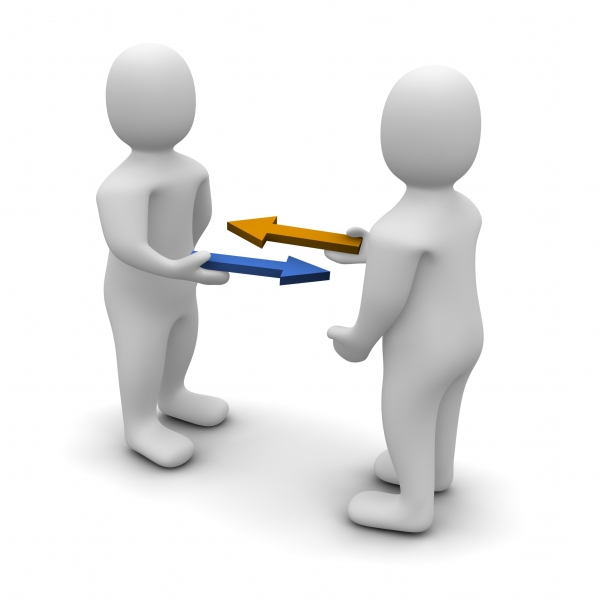
\includegraphics[scale=0.35]{troc4}
				\label{Visual Studio Code}
			\end{center}

		
	
		\vspace{3em}	
		\begin{tabular}{lll}
			\vspace{0.5em}
			 \textsc{\underline{Enseignants:}}	& \hspace{3em}	&	\textsc{\underline{Étudiants:}}		\\ 
			 \textsc{\textbf{\sc Bondiombouy carlyna }} & \hspace{15em}	&	\textsc{\textbf{\sc Gnoguem nestor}}	 \\				%\\ \vspace{1em}
			 \textsc{\textbf{\sc Valduriez patrick}}	& \hspace{15em}	&	\textsc{\textbf{\sc Houngue isaac}}	 \\				%\\ \vspace{1em}
													 	& \hspace{15em}	&	\textsc{\textbf{\sc Saibou aziz}}	 \\				%\\ \vspace{1em}
		\end{tabular}

		\vspace{6.7em}																
%		\fbox{\rule[-0.4cm]{0cm}{1cm} Une boite avec \verb!fbox! et avec \verb!rule!.}
		\textsc{\small Mars 2019}
		
		
	\end{center}
	
	\newpage
	\tableofcontents
	
	\newpage

	\section{\sc Introduction générale}
	\rule{1 \textwidth}{0.5pt} \textbf{}
	\vspace{2em}

		\subsection{ \sc Contexte}
		Le procédé qui consiste en l’abandon d’une chose  à quelqu’un dans le but d’avoir quelque chose en contrepartie est un échange dit \texttt{troc}.
		En plus de créer des relations ou tout simplement d'établir un contact humain solidaire, le \texttt{troc} permet à certains d'obtenir des objets ou de réaliser des projets qu'ils n'auraient pas pu acquérir sans cet échange de biens ou de savoir-faire. En outre, les objets que d'autres désirent jeter sont ainsi récupérés par un tiers, permettant la réduction de déchets et de donner à ceux qui en ont la nécessité. Les objets s'offrent une nouvelle vie au lieu d'être jetés inutilement et le pire, c'est que tout le monde est gagnant sans avoir débourser un seul euro. Un bon moyen de répartir le sourire aux lèvres. Par contre la difficulté de connaître de trouver des personnes avec qui troquer constitue la première limite de ce système d'échange. La  mise en place d'une plateforme de {\tt troc} s'affranchira de la limite citée ci haut et permettra un échange lucide renforçant les liens sociaux et réduisant le nombre d'objets qui prématurément, se retrouvent dans les décharges.
	
		
	
		\subsection{ \sc Problématique}
		
		
		Les système de {\tt troc} existant posent de grands problemes de confiances et ne sont ainsi confrontés qu'a la méfiance de la part des utilisateurs. Il faudra ainsi résoudre ce problème de confiance en implémentant dans notre système les principes de l'interaction homme-machine tels la robustesse, le guidage... La réussite de ce projet permettra aux populations de réduire la conservation des objets non utilisés ainsi que l'évacuation dans les décharges des objets qui auraient pu être utiles à d'autre personnes. 
	
	
	

		\subsection{ \sc Objectifs}
		Notre projet permettra à toute personne de trouver des gens avec qui troquer librement des objets. Nous devons dans ce projet rendre compte de la compréhension du \texttt{DataSet}, \texttt{BesoinEnData}. Toutefois,
			il n'est pas évident de reconnaître la nécessité ou non de l'utilisation des technologies du \texttt{BigData} dans les projets informatiques. %Il est donc utile de pratiquer (expérimenter) afin d'acquérir de l'expérience en ce qui concerne le choix des outils ou technologies du \texttt{Big Data}.
		 On doit ainsi rendre compte de la maîtrise des outils  soit des concepts suivants  et justifier nos choix des solutions (outils) que nous avons utilisé: \texttt{HDFS
		, Spark, Neo4J, MongoDB, DataSet}.
		
		\subsection{ \sc Plan du rapport}
		Partant de l'analyse et à la réalisation, on exposera toutes les différentes étapes nécéssaires à la construction de notre programme. Il suivra donc une conclusion résumant tout notre travail.
%		\rule{0.7 \textwidth}{2pt} \textbf{}

	\newpage
	 \section{\sc Description du projet}
	 \rule{1 \textwidth}{0.5pt} \textbf{}
	 
	 \vspace{2em}
	


	Le projet consiste en le developpement d'une plateforme pour les personnes intéressées par l'échange d'objets ({\tt troc}).	Notre système analysera les conditions de d'approbation ou de valiadtion du {\tt troc} entre deux ou plusieurs personnes.	 Les deux parties impliquées dans l'échange (les utilisateurs voulant échanger) doivent s'abonner à la plateforme avant de pouvoir utiliser notre service. Tout abonné peut ajouter des objets dans le but de l'echanger avec des objets qu'auront proposé d'autres abonnés. Un abonné serait donc en mesure de suggérer des objets contre ceux ou celui d'autres utilisateurs, qui les plaisent. A travers notre plateforme les abonnés relèverons leurs besoins sans affaiblir leur position de négociation. Cet avantage est important si l'abonné se trouve face à un monopole discriminant pour un bien très désiré.
	 
	 
	 
	  Nous pourrions tirer profit de ce projet en mettant en place des abonnements payants, des publicités ou des frais supplémentaires pour ceux qui veulent que leur objet soit bien placé sur la plateforme parmi les tops.
	

	


	\newpage
	\section{\sc Analyse et Conception}
		\rule{1 \textwidth}{0.5pt} \textbf{}
		
		\vspace{2em}
		L’analyse des besoins est une phase qui consiste à comprendre et à déterminer
		les différentes fonctionnalités et besoins du système.
		\subsection{\sc Identification des acteurs}
		L'identification des acteurs d'une application est une phase primordial de l'analyse des besoins, c'est ainsi qu'on a pu identifier les acteurs suivants:
		\begin{description}
			\item [\sc Client:] Toute personne physique capable de poster ou de consulter un objet.
			\item[\sc Administrateur:] Toute personne susceptible de maintenir le système du point de vue gestion des compte des utilisateurs.
		\end{description}
	\subsection{\sc Les besions fonctionnels du système}
		 Les besoins fonctionnels constituent les fonctionnalités que le système devra assurer, parmi les
		 quelles, nous décrivons principalement les fonctions suivantes: 
		 \begin{enumerate}
		 	\item Consulter des objets
		 	\item Troquer un objet
		 	\item Ajouter un objet
		 \end{enumerate}
		 Le diagramme des cas d'utilisation suivant rend compte des fonctionnalités de notre application
			\begin{center}
				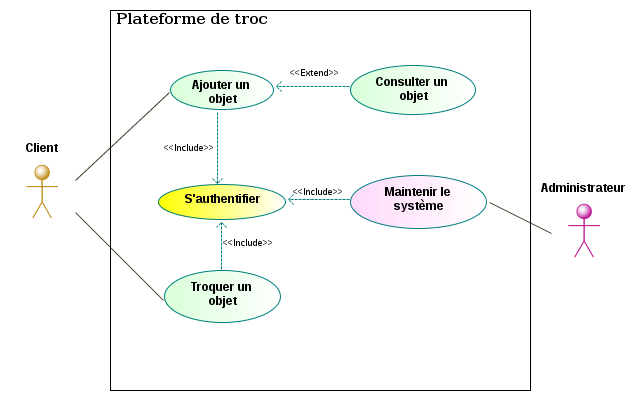
\includegraphics[scale=1, width=\textwidth, height=8cm]{usecase}
				\label{usecase}
			\end{center}
		\subsection{\sc Modèle dynamique}
			Après la description des différents cas d’utilisation, nous allons élaborer le modèle dynamique
			dans lequel nous allons décrire les scénarios de quelques cas d’utilisations les plus importants sous forme de diagrammes de séquence.
			
			\begin{center}
			
				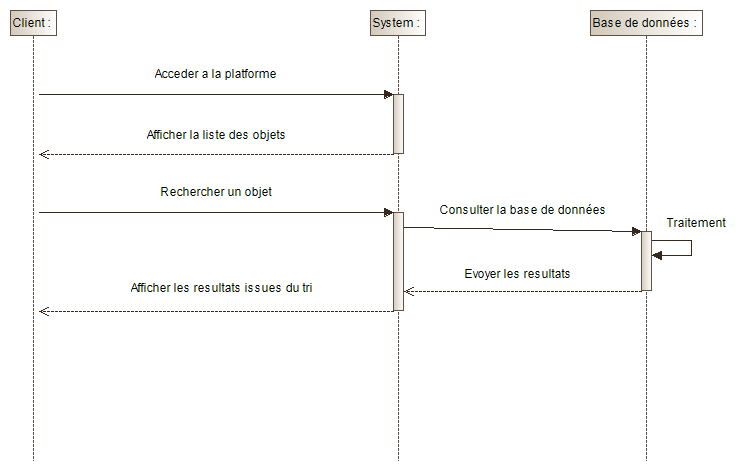
\includegraphics[scale=1, width=0.8\textwidth, height=10cm]{troc0}
				\label{troc0}
			\end{center}
		La figure précédente est celui du diagramme de séquence est du cas "Rechercher un objet"
			\begin{center}
				
				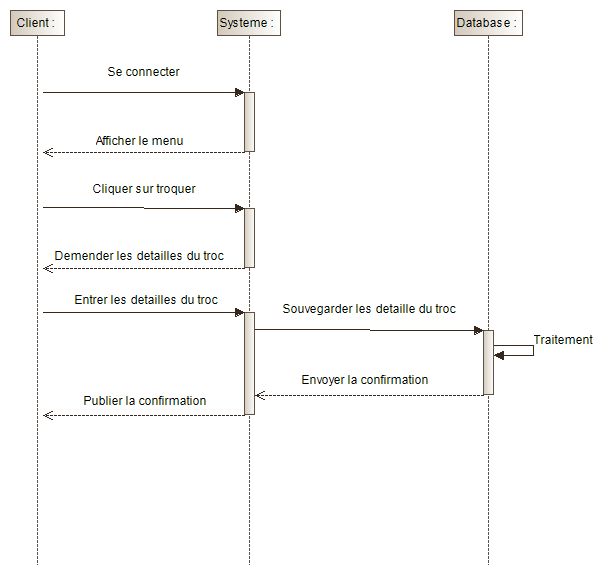
\includegraphics[scale=1, width=0.8\textwidth, height=10cm]{troc1}
				
				\label{troc1}
			\end{center}
			La figure précédente est celui du diagramme de séquence est du cas "Ajouter un objet"
			\begin{center}
			
				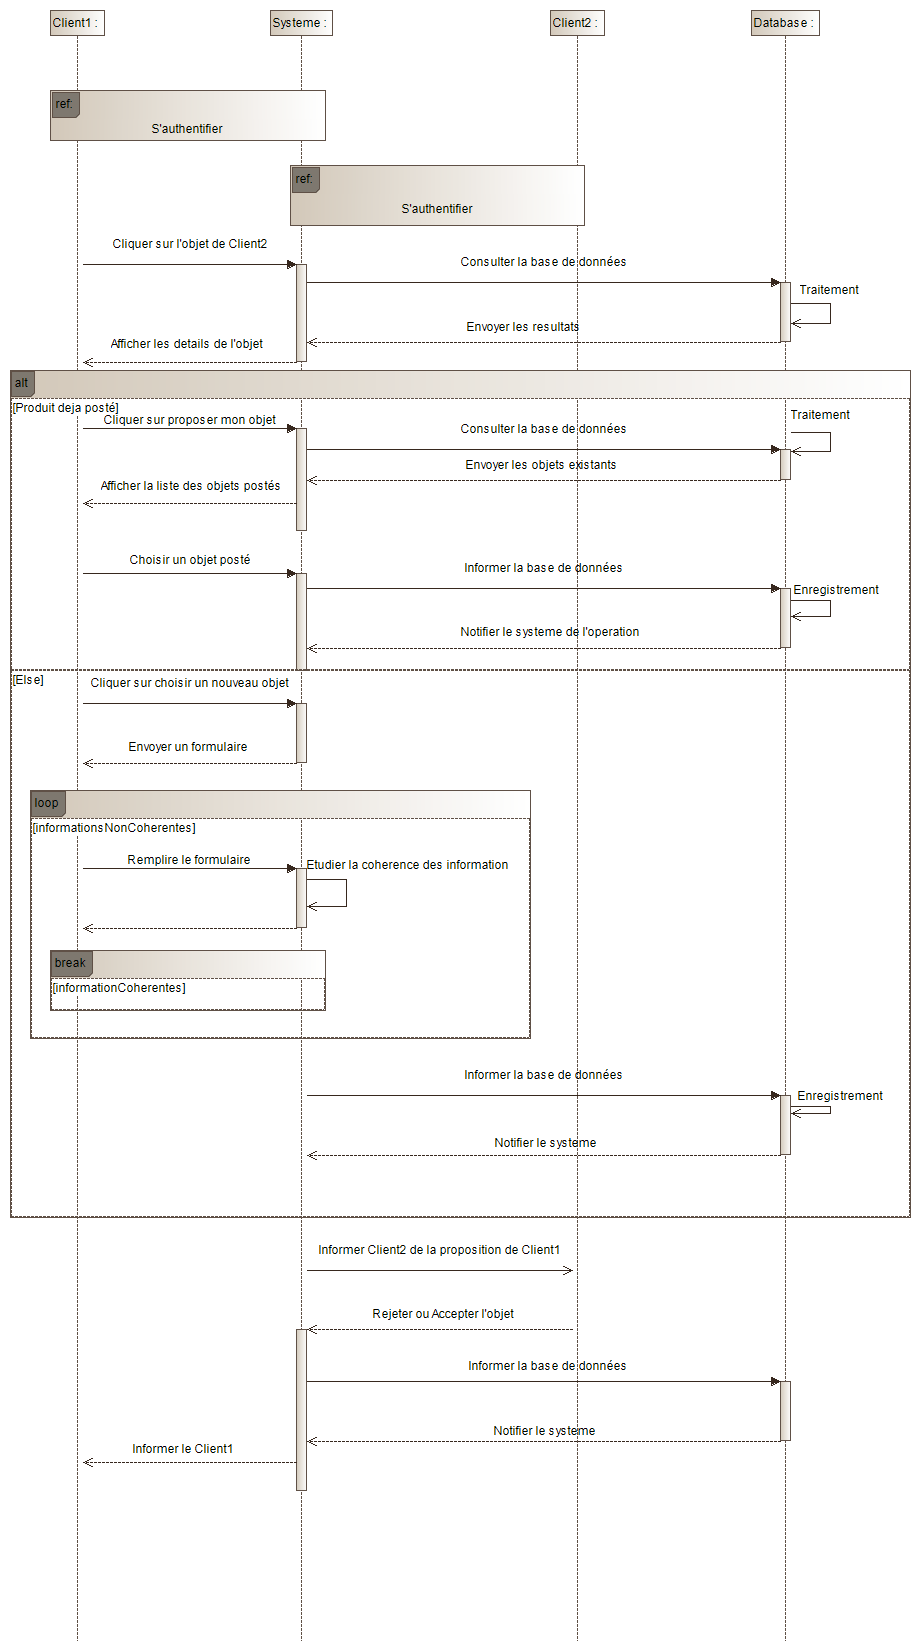
\includegraphics[scale=1, width=0.8\textwidth, height=20cm]{troc6}
			
				\label{troc6}
			\end{center}
		La figure précédente est celui du diagramme de séquence est du cas "Troquer un objet"
		
		\vspace{2em}
			
	Le diagramme de classe dictant le comportement de notre programme est le suivant:
		 	\begin{center}
		 	
		 		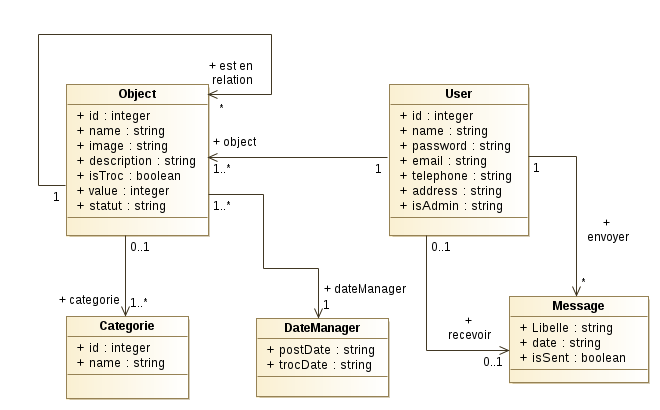
\includegraphics[scale=1, width=0.9\textwidth, height=10cm]{class}
		 		
		 		\label{class}
		 	\end{center}
	 
	
	
	\newpage
	\section{\sc Réalisation}
		\rule{1 \textwidth}{0.5pt} \textbf{}
		\vspace{2em}
		\subsection{\sc DataSet vs Besoin en données}
			Vu que le caractère des objets à échanger n'est pas prédéfini, on doit s'attendre à une grande variété presque imprevisible de données de la part des client. Pensant la plateforme à une échelle mondiale, il y aura tout de même la vitesse de génération des données qui deviendra un facteur déterminant dans le choix des solutions le long de la phase de développement de notre plateforme. 
			
			Non seulement notre système implemente les trois premiers {\tt \_V\_} de la théorie du {\tt BigData} ({\it volume, velocity veracity}), mais aussi, le concept de valorisation des données en {\tt BigData} (utilisation des données pour en extraire de la valeur) à des fin publicitaires par exemple, nous motive à opter pour une solution {NoSQL} en ce qui concerne le stockage et la gestion de nos données.
			
			\subsubsection{ \bf {\sc Choix du sgbd NoSQL}}
			
			MongoDB est un sgbd orienté document. 
			Il repose sur le principe du clé/valeur, mais avec une extension sur les champs qui composent ce document.
			Il propose ainsi un language  d'interrogation riche permettant de faire des manipulations complexes sur chaque attribut du document (et sous-documents) comme dans une base de données traditionnelles, tout en passant à l'échelle dans un contexte distribué.
			
			Considerons le sgbd {\tt Spark}, cette solution est moins appropriée pour la lecture de données spécifiques comme pour les clés/valeurs, ce qui ne nous motive pas à l'utiliser.
			
		
			
			De la même façon, {\tt Neo4j} est une solution utilisée dans les systèmes ou la gestion de chemins, de propagations est une priorité.  
			
		On a ainsi choisi {\tt MongoDB}.
		
		\subsubsection{\sc Présentation du dataset}
			
		Pour mieux apréhender le comportement de notre système il est tres utile que les données de test ({\tt DataSet}) lors de la phase de développement soient considérables et cohérentes avant d'entrer en production. Nous avons donc utiliser le {\tt DataSet} inspiré de notre diagramme de classe et contenu dans le fichier {\tt dataset.json} annexé à notre rapport.
		

		
	\subsection{\sc Environnement de développement logiciel}

	
	
	
	En vue d'écrire un programme cohérent très tôt comprehensible par nous même et eventuellement par d'autres développeurs en vue d'une maintenance tres aisée, nous avons adopté la structuration suivante pour nos  fichiers. 
	\begin{center}
		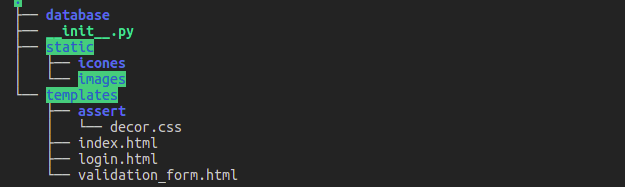
\includegraphics[scale=1, width=0.8\columnwidth]{archi}
	\end{center}
	
	\begin{enumerate}
		\item Le dossier {\tt static} contient les données static de notre application
		\item Le dossier {\tt templates} contient les templates de notre application	
		\item Le dossier {\tt assert} contient tous les fichiers de styles ({\tt .css}) de notre application.
		\item Le dossier {\tt images}  sous le dossier {\tt static} contient toutes les images des objets de notre application.
		\item Le dossier {\tt icones} sous le dossier {\tt static}
	\end{enumerate}
	
\subsubsection{\sc Les outils logiciels que nous avons utilisé sont les suivants}
	\begin{description}
		\item[\sc Modelio 3.7:] Un logiciel de modélisation open-source
				\begin{center}
					
\includegraphics[scale=1, width=0.56\textwidth, height=4cm]{modelio}
					\label{modelio}
				\end{center}
		
		\item[\sc Visual-Studio-Code 1.28:] Un éditeur de texte avancé
				\begin{center}
					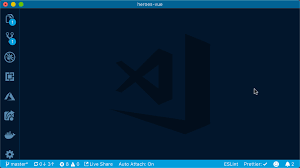
\includegraphics[scale=1, width=0.5\textwidth, height=5cm]{vscode}
					\label{vscode}
				\end{center}
		\item[\sc Flask 1.0:]  Un \textit{mini-framework} open-source de développement web en Python
		
				\begin{center}
					
\includegraphics[scale=1, width=0.5\textwidth, height=4cm]{flask}
					\label{flask}
				\end{center}
		\item[\sc Jinja2:] Un moteur de template
			\begin{center}
				
\includegraphics[scale=1, width=0.5\textwidth, height=4cm]{jinja}
				\label{jinja}
			\end{center}
			
		\item[\sc Mongo-DB:] Un système de gestion de base de données orienté document open-source developpé en {\tt C++}
			\begin{center}
				
\includegraphics[scale=1, width=0.5\textwidth, height=4cm]{mongo}
				\label{mongo}
			\end{center}
		
		\item [\sc \href{https://www.mockaroo.com/}{\color{blue} Mockaroo:}  ] Une plateforme de génération de données. Nous l'avons utilisé pour pour générer notre {\tt DataSet}  
		
		\begin{center}
			
\includegraphics[scale=1]{mock}
			\label{mock}
		\end{center}
	\end{description}
	
	\subsection{\sc Quelques interfaces de notre application}
	
	Voici quelques interfaces de notre application:
	\begin{center}
		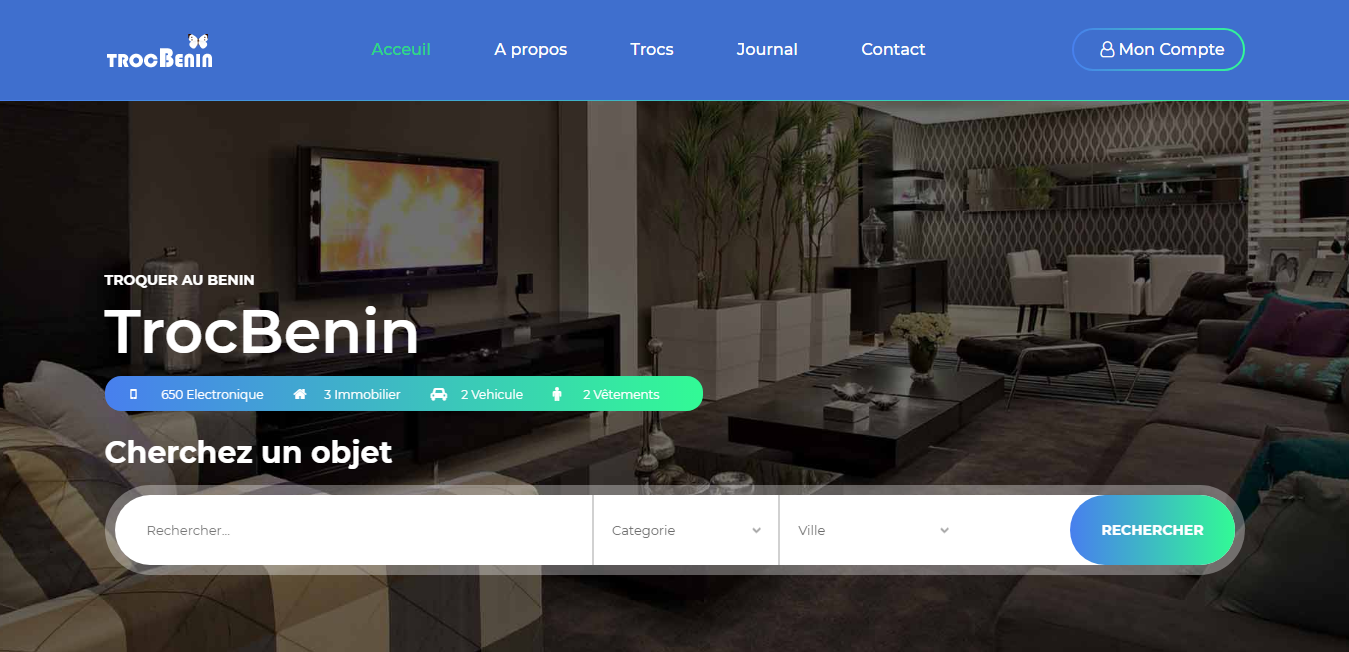
\includegraphics[scale=0.5, height=8cm]{inter1}
	\end{center}
	
	L'interface précedente est la page d'acceuil de l'application. Le client a possibilité de rechercher un objet.
	


\begin{center}
	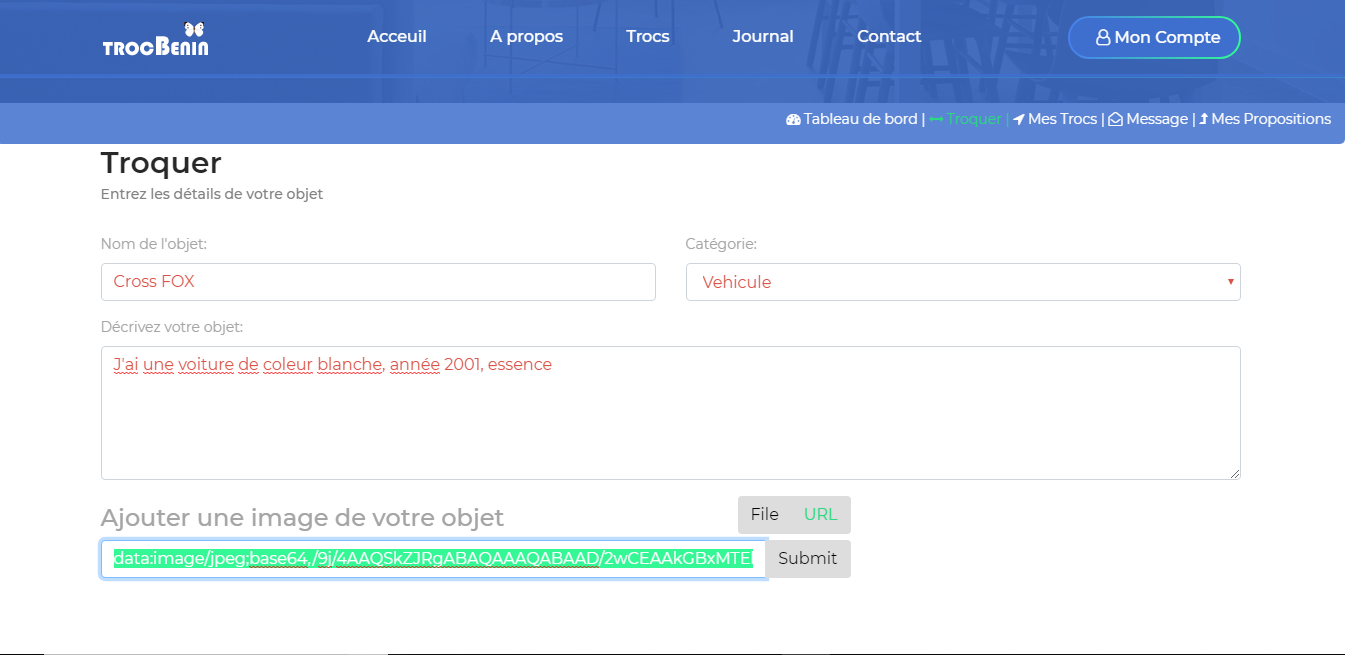
\includegraphics[scale=0.5, height=8cm]{troquer}
\end{center}
	L'interface précédente est la page permettant aux utilisateurs d'ajouter un objet pour un {\tt troc}
	
	\subsection{\sc Démonstration}
	
	

	\newpage
	\section{\sc Conclusion}
		\rule{1 \textwidth}{0.5pt} \textbf{}
		\vspace{2em}
		
	Dans la première partie de ce travail, nous avons introduit une plateforme permettant à ses utilisateurs d’échanger des objets. Cette plateforme sera utilisée au Bénin. Dans la deuxième partie, nous présentons avec plus de précision le contexte du projet. Après avoir examiné le contexte, nous avons modélisé le projet à l'aide de diagrammes UML dans la troisième section. Nous avons présenté quatre cas d'utilisation. le client utilise le système pour ajouter un objet, échanger un objet et rechercher un objet offert en échange. L'administrateur mentien le systeme. Nous avons présenté la séquence des interactions impliquées dans ces quatre cas d'utilisation ainsi qu'un diagramme de classes montrant les différentes entités sous forme de classes impliquées dans notre système. Dans la quatrième section, nous avons présenté notre choix de technologies de mise en œuvre et notre data set. Nous avons choisi MongoDB sur Spark et Neo4J parce qu’il propose un langage de requête riche permettant d’effectuer des manipulations complexes sur chaque attribut du document. Nous avons ensuite présenté quelques captures d'écran de la hiérarchie des fichiers de notre projet et quelques captures d'interface.
	%	\newpage
	%	\begin{center}
	%		{\large \sc DataSet}
	%	\end{center}
			
%				\lstinputlisting[ firstline=1]{dataset.json}\label{dataset}
\end{document}